\def\ktitle{ARM ASSIGNMENT}
\def\kauthor{Chakali Suresh}
\def\kcontact{chakalisuresh2223@gmail.com}
\def\kmodule{IITH - Future Wireless Communication}
%\renewcommand{\thesection}{\arabic{section}}
%\renewcommand{\thesubsection}{\arabic{subsection}}
%\titleformat{\subsubsection}{\normalfont\itshape\filcenter}{\thesubsubsection}{1em}{}
\documentclass[journal,12pt,twocolumn]{IEEEtran}
\usepackage{enumitem}
%\renewcommand{\thesection}{\arabic{section}}
%\renewcommand{\thesubsection}{\arabic{subsection}}
\usepackage{tikz}
\usepackage{circuitikz}
\usepackage{karnaugh-map}
\usepackage{tabularx}
\usepackage{circuitikz}
\usepackage{tikz}
\usepackage{titlesec}
\usepackage{multirow}
\title{\ktitle}
\author{\kauthor\\\kcontact\\\kmodule}
\begin{document}
\maketitle
\tableofcontents
\section{\textbf{Question}}
 The digital circuit shown \rule{9mm}{0.4pt}
\begin{figure}[ht]
    \centering
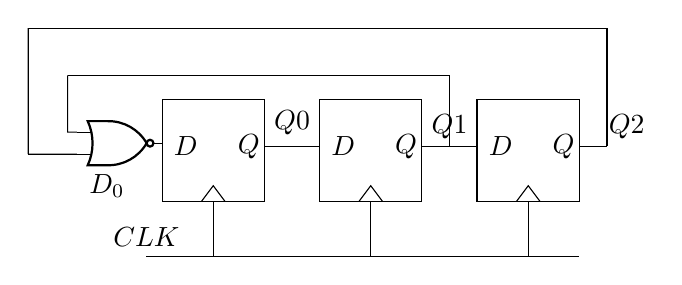
\begin{tikzpicture}
\ctikzset{                                   
logic ports=ieee,                   
logic ports/scale=0.5               
}                                    
\draw(-1.3,-0.56)node[nor port,anchor=out](x) {};  
%Drawing flip-flops
\draw (-1.3,-1.3) rectangle (0,0);
\draw(-1,-0.6) node{$D$};
\draw(-2,-1.1) node{$D_0$};
\draw(-0.2,-0.6) node{$Q$};
\draw(0.7,-1.3) rectangle (2,0);
\draw(1,-0.6) node{$D$};
\draw(1.8,-0.6) node{$Q$};
\draw(2.7,-1.3) rectangle (4,0);
\draw(3,-0.6) node{$D$};
\draw(3.8,-0.6) node{$Q$};
%connecting them
\draw(0,-0.6) -- (0.7,-0.6);
\draw(2,-0.6) -- (2.7,-0.6);
\draw(4,-0.6) -- (4.35,-0.6);
%drawing clk
\draw(-1.5,-2) node[above]{$CLK$} -- (3.35,-2);
%connecting clk 
\draw(-0.65,-2) -- (-0.65,-1.3);
\draw(1.35,-2) -- (1.35,-1.3);
\draw(3.35,-2) -- (3.35,-1.3);
\draw(3.35,-2) -- (4,-2);
%drawing clk edges
\draw(-0.5,-1.3) -- (-0.65,-1.1) -- (-0.8,-1.3);
\draw(1.2,-1.3) -- (1.35,-1.1) -- (1.5,-1.3);
\draw(3.2,-1.3) -- (3.35,-1.1) -- (3.5,-1.3);
%drawing Q2,Q1,Q0
%\draw(0.35,-0.6) --(0.35,0.2);
\draw(2.35,-0.6) --(2.35,0.3);
\draw(4.35,-0.6) --(4.35,0.9);
\draw(4.35,0.9) -- (-3,0.9);
\draw(2.35,0.3) -- (-2.5,0.3);
\draw(x.in 2) -|(-3,-0.7)to[short](-3,0.9);
\draw(x.in 1) -|(-2.5,-0.3)to[short](-2.5,0.3);
\draw(0.35,-0.3)node{$Q0$};
\draw(2.35,-0.35)node{$Q1$};
\draw(4.6,-0.35)node{$Q2$};
\end{tikzpicture}
   % \caption{Caption}
\end{figure}
\section{\textbf{Answer}}
The above question can be solved by using Truth Table and karnaugh-map.
\subsection{\centering Truth Table}
\begin{tabularx}{0.45\textwidth}{
 | >{\centering\arraybackslash}X
 | >{\centering\arraybackslash}X
 | >{\centering\arraybackslash}X
 | >{\centering\arraybackslash}X
 | >{\centering\arraybackslash}X
 | >{\centering\arraybackslash}X
        | >{\centering\arraybackslash}X
        | >{\centering\arraybackslash}X
        | >{\centering\arraybackslash}X|}
    \hline
  \multicolumn{3}{|c|}{Present State}&\multicolumn{3}{c|}{Flip-Flop i/p}&\multicolumn{3}{c|}{Next State}\\ 
    \hline
\textbf{$Q_0$}&\textbf{$Q_1$}&\textbf{$Q_2$}&\textbf{$D_0$}&\textbf{$D_1$}&\textbf{$D_2$}&\textbf{$Q_0'$}&\textbf{$Q_1'$}&\textbf{$ Q_2'$}\\
 \hline
 0&0&0&1&0&0&1&0&0\\
 \hline
 1&0&0&1&1&0&1&1&0\\
 \hline
        1&1&0&0&1&1&0&1&1\\
 \hline
 0&1&1&0&0&1&0&0&1\\
 \hline
 0&0&1&0&0&0&0&0&0\\
 \hline
 \end{tabularx}
\begin{figure}
\subsection{\centering K-Map Implentation}
\resizebox{0.45\textwidth}{!}{%
 \begin{karnaugh-map}[4][2][1][$Q_1Q_2$][$Q_0$]
  \maxterms{1,2,3,5,6,7}
  \minterms{4,0}
  \implicant{0}{4}
  %\implicant{4}{12}
  %\implicantedge{12}{12}{14}{14}
 \end{karnaugh-map}%
}
 \centering \textbf{ $D_0$ = $\overline Q_1 +  \overline Q_2$}
\resizebox{0.45\textwidth}{!}{%
 \begin{karnaugh-map}[4][2][1][$Q_1Q_2$][$Q_0$]
  \maxterms{1,2,3,5,0,7}
  \minterms{4,6}
  \implicantedge{4}{4}{6}{6}
  %\implicant{4}{12}
  %\implicantedge{12}{12}{14}{14}
 \end{karnaugh-map}%
}
\centering \textbf{ $D_1$ = $Q_0$}
\resizebox{0.45\textwidth}{!}{%
 \begin{karnaugh-map}[4][2][1][$Q_1Q_2$][$Q_0$]
  \maxterms{1,2,4,5,0,7}
  \minterms{3,6}
  \implicant{3}{3}
            \implicant{6}{6}
  %\implicant{4}{12}
  %\implicantedge{12}{12}{14}{14}
 \end{karnaugh-map}%
}
	\centering \textbf{ $D_2$ = $Q_1$ }
\end{figure}
 \vspace{\baselineskip}
Therefore, given circuit is Divide by 5 circuit.
 \section{\textbf{Components}}
 \begin{tabularx}{0.45\textwidth}{
   | >{\centering\arraybackslash}X
   | >{\centering\arraybackslash}X
   | >{\centering\arraybackslash}X |
   }
   \hline
   \textbf{Components}&\textbf{Values}&\textbf{Quantity}\\
   \hline
   VAMAN &  & 1\\
   \hline
   Jumper Wires & M-M & 25\\
   \hline
   Breadboard & & 1\\
   \hline
                LED & & 4\\
                \hline
                Resistor & &\\
                \hline
                Flip Flop & 7474 & 2 \\
\hline  
 \end{tabularx}
\section{\textbf{Implementation}}
\begin{tabular}{|c|c|c|c|c|c|c|c|c|c|c|c|c|}      
\hline                              
\multirow{2}{*}{} & \multicolumn{3}{c|}{INPUT} & \multicolumn{3}{c|}{OUTPUT} & \multicolumn{2}{c|}{\multirow{2}{*}{CLOCK}} & \multicolumn{4}{c|}{\multirow{2}{*}{5V}} \\      
\cline{2-7}     
& Q0 & Q1 & Q2 & Q0' & Q1' & Q2' & \multicolumn{2}{|c|}{\multirow{2}{*}{}} & \multicolumn{4}{c|}{} \\        
\hline          
VAMAN(pins) & 2 & 3 & 4 & 18 & 21 & 22 & \multicolumn{2}{c|}{5} &
\multicolumn{4}{c|}{\multirow{3}{*}{}}\\                                   
\hline                             
7474 & 5 & 9 &  & 2 & 12 &  & CLK1 & CLK2 & 1 & 4 & 10 & 13 \\                   
\hline                     
7474 & & & 9 & & & 12 & CLK1 & CLK2 & 1 & 4  & 10 & 13 \\                       
\hline                         
        
\end{tabular}
\begin{center}
    Connections
\end{center}
\textbf{Procedure}
\begin{enumerate}[label={\arabic*}.]
 \item Connect the circuit as per the above table.
 \item Connect LEDs to the output pins of the VAMAN to see output.
 \item Execute the circuit using the below code.
  \vspace{\baselineskip}\\
                \begin{tabularx}{0.45\textwidth}{
    | >{\centering\arraybackslash}X|}
   \hline
https://github.com/Chakali23/FWC\\/tree/main/IDE/arm(VAMAN)\\
   \hline
  \end{tabularx}\\
  \end{enumerate}
\end{document}
